\documentclass[12pt, twoside]{article}
\usepackage[francais]{babel}
\usepackage[T1]{fontenc}
\usepackage[latin1]{inputenc}
\usepackage[left=7mm, right=7mm, top=7mm, bottom=7mm]{geometry}
\usepackage{float}
\usepackage{graphicx}
\usepackage{array}
\usepackage{multirow}
\usepackage{amsmath,amssymb,mathrsfs}
\usepackage{soul}
\usepackage{textcomp}
\usepackage{eurosym}
 \usepackage{variations}
\usepackage{tabvar}

\begin{document}


\section*{\center{Aide individualis�e: Statistiques descriptives}}

\subsection*{Exercice 1}

Pour les deux �nonc�s ci-dessous, dire si les affirmations sont vraies ou
fausses.

\enskip

\begin{tabular}{cc}
\begin{minipage}{9cm}
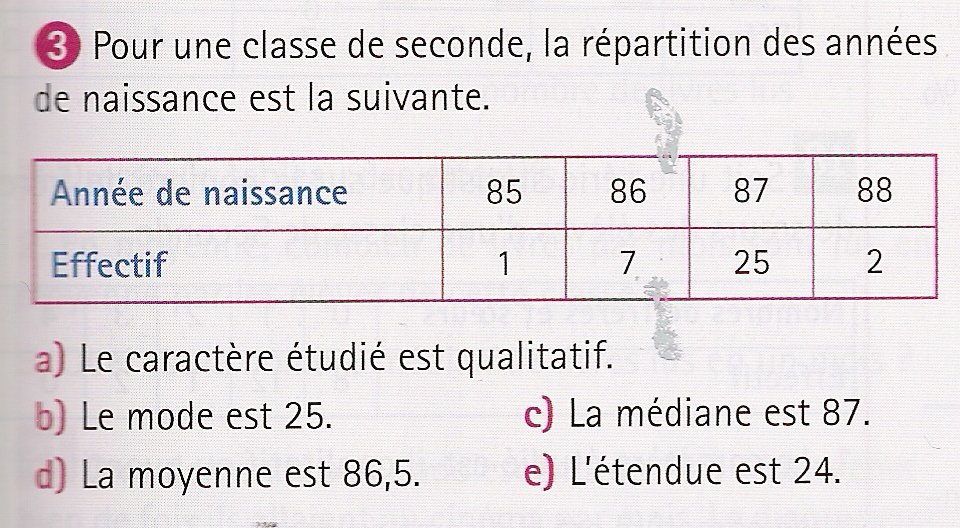
\includegraphics[width=9cm]{images/vrai_faux1.jpg}
\end{minipage}
&
\begin{minipage}{9cm}
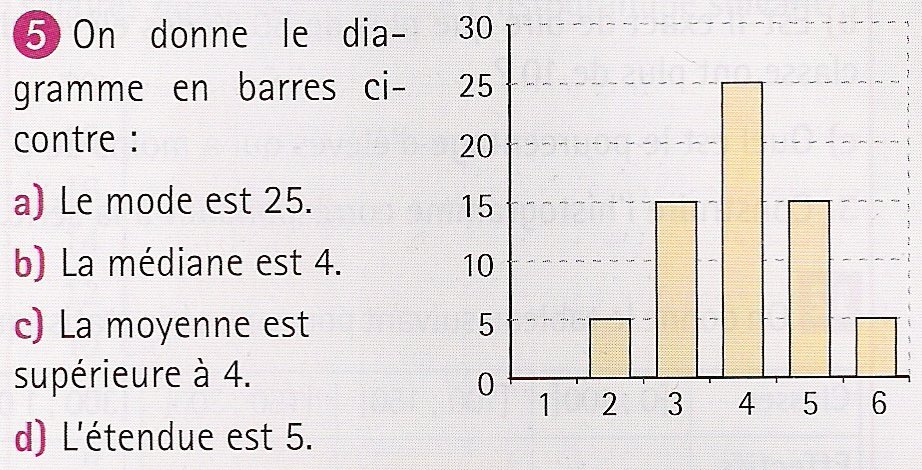
\includegraphics[width=9cm]{images/vrai_faux2.jpg}
\end{minipage}
\end{tabular}


\subsection*{Exercice 2}

Apr�s une s�rie de 3 contr�les, un �l�ve a une moyenne de 11. Il obtient 15 au
contr�le suivant. Toutes les notes sont
coefficient 1. Calculer sa nouvelle moyenne (on pourra faire un sch�ma).


\subsection*{Exercice 3}

Maud veut calculer rapidement sa moyenne, ses notes sont:
10 \quad 12 \quad 14 \quad 7.5 \quad 13 \quad 9.5 \quad 11 \quad 15.

Maud enl�ve 10 � chaque note; elle calcule la moyenne $\bar{y}$ des nombres
obtenus puis rajoute 10 pour obtenir sa moyenne.

\begin{enumerate}
  \item Effectuer le calcul de Maud.
  \item Citer la propri�t� utilis�e.
  \item Calculer de m�me la moyenne de Valentin: 
  9 \quad 8.5 \quad 16 \quad 7.5 \quad 12 \quad 10.5 
\end{enumerate}


\subsection*{Exercice 4}

Dans une grande entreprise, on a interrog� les salari�s
afin de conna�tre la dur�e de leurs pauses d�jeuners.

On donne l'histogramme suivant:
\begin{center}
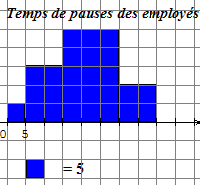
\includegraphics[width=5cm]{images/histo.png}
\end{center}


\begin{enumerate}
  \item Quelles sont les classes de cette s�rie?
  \item Repr�senter la s�rie sous forme de tableau.
  \item D�terminer la m�diane de la s�rie.
\end{enumerate} 
\end{document}
